\section{Host et Controller}


\begin{frame}
	\frametitle{Architecture physique}
	\begin{block}{Host et controller séparés}
		\begin{minipage}[t]{0.48\linewidth}
		\begin{figure}
			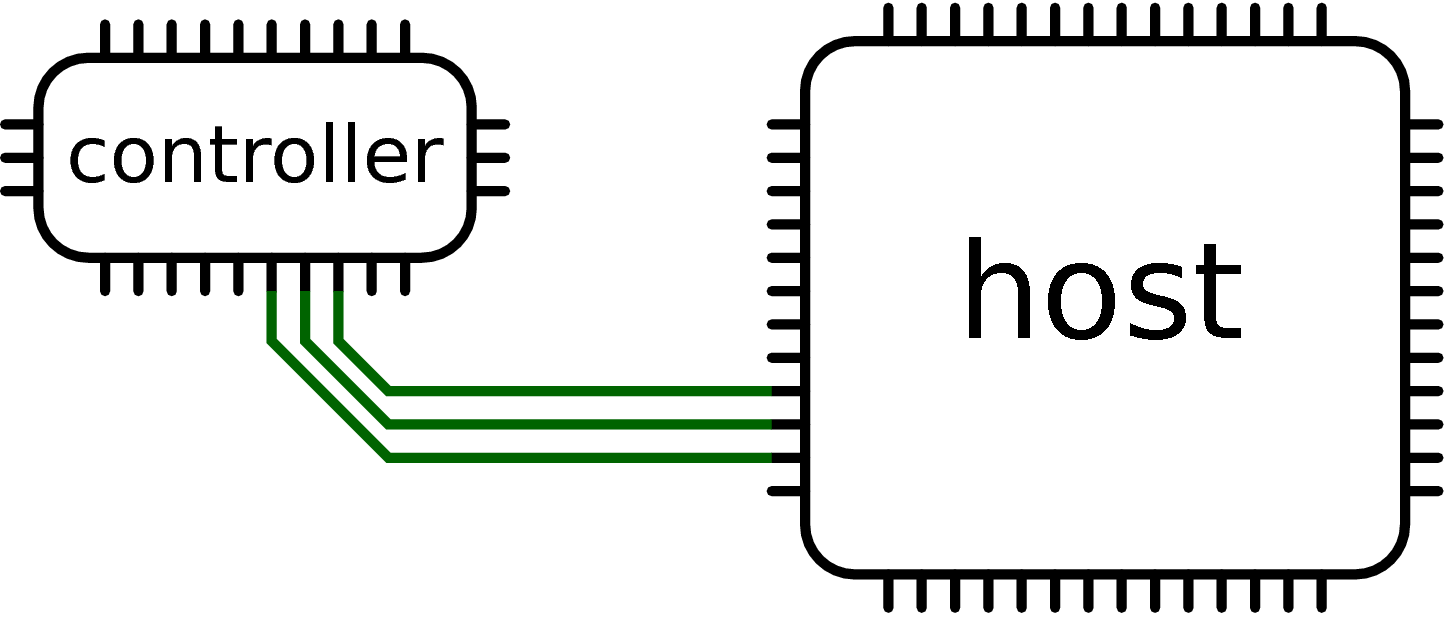
\includegraphics[width=4cm]{img/HC_sep.png}
		\end{figure}
		\end{minipage}
		\begin{minipage}[t]{0.48\linewidth}
		\begin{figure}
			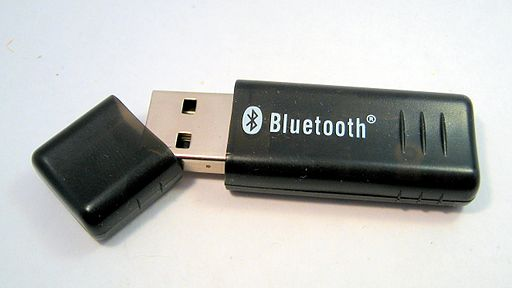
\includegraphics[width=3cm]{img/dongle.jpg}
		\end{figure}
		\end{minipage}
	\end{block}
	\begin{block}{System on a Chip}
		\begin{minipage}[t]{0.48\linewidth}
		\begin{figure}
			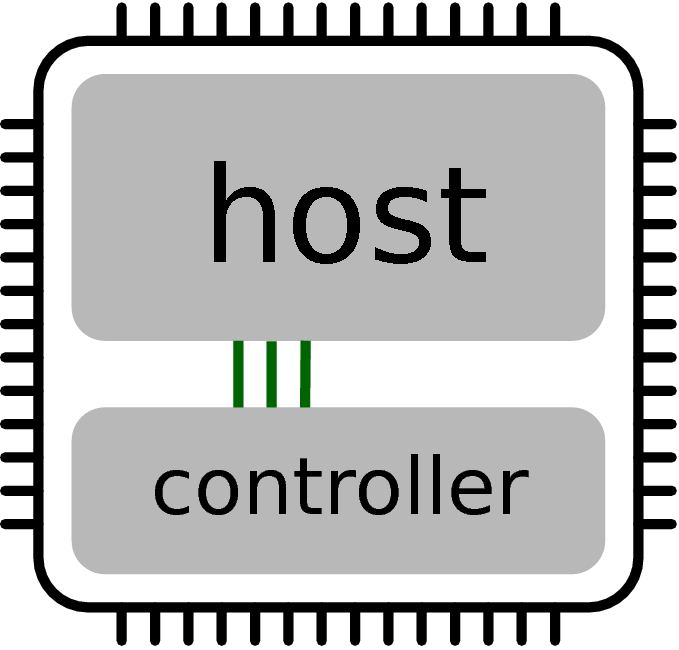
\includegraphics[width=2cm]{img/HC_soc.png}
		\end{figure}
		\end{minipage}
		\begin{minipage}[t]{0.48\linewidth}
		\begin{figure}
			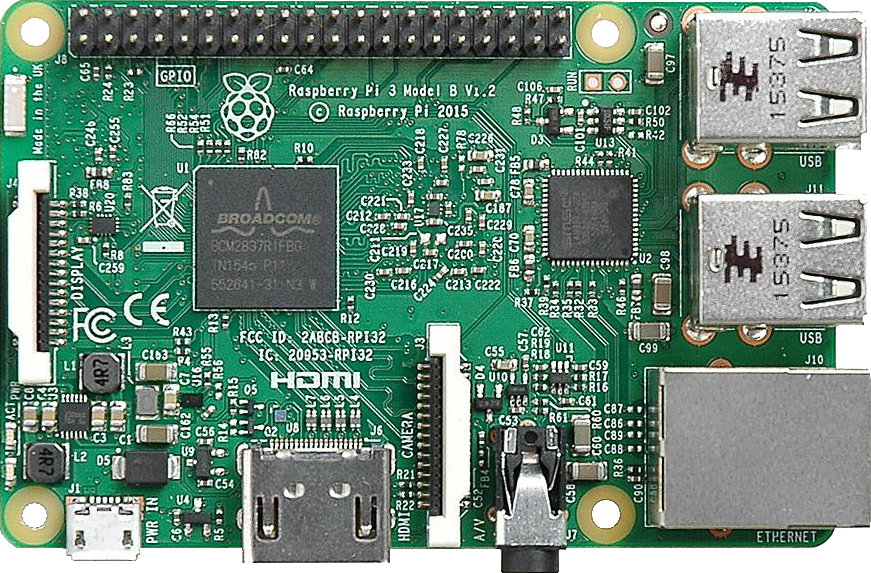
\includegraphics[width=3cm]{img/rpi3.png}
		\end{figure}
		\end{minipage}
	\end{block}
\end{frame}

\begin{frame}
	\frametitle{Standard Bluetooth}
	\center{\textbf{Services}, \textbf{Profils} et \textbf{Protocoles}}
	\vspace{0.5cm}
	\begin{itemize}
		\item Liaison physique
		\item Adressage physique
		\item Controle de flux
		\item Multiplexage
		\item Chiffrement
		\item Protocoles over Bluetooth
		\item "Profils"
	\end{itemize}
	\vspace{0.5cm}
	\tiny{\url{https://www.bluetooth.com/specifications/adopted-specifications}}
\end{frame}


\begin{frame}
	\frametitle{Architecture logique}
\end{frame}

\begin{frame}
	\frametitle{Controller}
\end{frame}

\begin{frame}
	\frametitle{Host}
\end{frame}

\begin{frame}
	\frametitle{Canaux de communication}
\end{frame}

